\documentclass[1p]{elsarticle_modified}
%\bibliographystyle{elsarticle-num}

%\usepackage[colorlinks]{hyperref}
%\usepackage{abbrmath_seonhwa} %\Abb, \Ascr, \Acal ,\Abf, \Afrak
\usepackage{amsfonts}
\usepackage{amssymb}
\usepackage{amsmath}
\usepackage{amsthm}
\usepackage{scalefnt}
\usepackage{amsbsy}
\usepackage{kotex}
\usepackage{caption}
\usepackage{subfig}
\usepackage{color}
\usepackage{graphicx}
\usepackage{xcolor} %% white, black, red, green, blue, cyan, magenta, yellow
\usepackage{float}
\usepackage{setspace}
\usepackage{hyperref}

\usepackage{tikz}
\usetikzlibrary{arrows}

\usepackage{multirow}
\usepackage{array} % fixed length table
\usepackage{hhline}

%%%%%%%%%%%%%%%%%%%%%
\makeatletter
\renewcommand*\env@matrix[1][\arraystretch]{%
	\edef\arraystretch{#1}%
	\hskip -\arraycolsep
	\let\@ifnextchar\new@ifnextchar
	\array{*\c@MaxMatrixCols c}}
\makeatother %https://tex.stackexchange.com/questions/14071/how-can-i-increase-the-line-spacing-in-a-matrix
%%%%%%%%%%%%%%%

\usepackage[normalem]{ulem}

\newcommand{\msout}[1]{\ifmmode\text{\sout{\ensuremath{#1}}}\else\sout{#1}\fi}
%SOURCE: \msout is \stkout macro in https://tex.stackexchange.com/questions/20609/strikeout-in-math-mode

\newcommand{\cancel}[1]{
	\ifmmode
	{\color{red}\msout{#1}}
	\else
	{\color{red}\sout{#1}}
	\fi
}

\newcommand{\add}[1]{
	{\color{blue}\uwave{#1}}
}

\newcommand{\replace}[2]{
	\ifmmode
	{\color{red}\msout{#1}}{\color{blue}\uwave{#2}}
	\else
	{\color{red}\sout{#1}}{\color{blue}\uwave{#2}}
	\fi
}

\newcommand{\Sol}{\mathcal{S}} %segment
\newcommand{\D}{D} %diagram
\newcommand{\A}{\mathcal{A}} %arc


%%%%%%%%%%%%%%%%%%%%%%%%%%%%%5 test

\def\sl{\operatorname{\textup{SL}}(2,\Cbb)}
\def\psl{\operatorname{\textup{PSL}}(2,\Cbb)}
\def\quan{\mkern 1mu \triangleright \mkern 1mu}

\theoremstyle{definition}
\newtheorem{thm}{Theorem}[section]
\newtheorem{prop}[thm]{Proposition}
\newtheorem{lem}[thm]{Lemma}
\newtheorem{ques}[thm]{Question}
\newtheorem{cor}[thm]{Corollary}
\newtheorem{defn}[thm]{Definition}
\newtheorem{exam}[thm]{Example}
\newtheorem{rmk}[thm]{Remark}
\newtheorem{alg}[thm]{Algorithm}

\newcommand{\I}{\sqrt{-1}}
\begin{document}

%\begin{frontmatter}
%
%\title{Boundary parabolic representations of knots up to 8 crossings}
%
%%% Group authors per affiliation:
%\author{Yunhi Cho} 
%\address{Department of Mathematics, University of Seoul, Seoul, Korea}
%\ead{yhcho@uos.ac.kr}
%
%
%\author{Seonhwa Kim} %\fnref{s_kim}}
%\address{Center for Geometry and Physics, Institute for Basic Science, Pohang, 37673, Korea}
%\ead{ryeona17@ibs.re.kr}
%
%\author{Hyuk Kim}
%\address{Department of Mathematical Sciences, Seoul National University, Seoul 08826, Korea}
%\ead{hyukkim@snu.ac.kr}
%
%\author{Seokbeom Yoon}
%\address{Department of Mathematical Sciences, Seoul National University, Seoul, 08826,  Korea}
%\ead{sbyoon15@snu.ac.kr}
%
%\begin{abstract}
%We find all boundary parabolic representation of knots up to 8 crossings.
%
%\end{abstract}
%\begin{keyword}
%    \MSC[2010] 57M25 
%\end{keyword}
%
%\end{frontmatter}

%\linenumbers
%\tableofcontents
%
\newcommand\colored[1]{\textcolor{white}{\rule[-0.35ex]{0.8em}{1.4ex}}\kern-0.8em\color{red} #1}%
%\newcommand\colored[1]{\textcolor{white}{ #1}\kern-2.17ex	\textcolor{white}{ #1}\kern-1.81ex	\textcolor{white}{ #1}\kern-2.15ex\color{red}#1	}

{\Large $\underline{12n_{0215}~(K12n_{0215})}$}

\setlength{\tabcolsep}{10pt}
\renewcommand{\arraystretch}{1.6}
\vspace{1cm}\begin{tabular}{m{100pt}>{\centering\arraybackslash}m{274pt}}
\multirow{5}{120pt}{
	\centering
	\includegraphics[width=112pt]{../../../GIT/diagram.site/Diagrams/png/2304_12n_0215.png}\\
\ \ \ A knot diagram\footnotemark}&
\allowdisplaybreaks
\textbf{Linearized knot diagam} \\
\cline{2-2}
 &
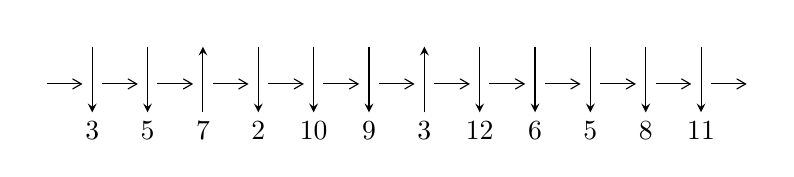
\begin{tikzpicture}[x=20pt, y=17pt]
	% nodes
	\node (C0) at (0, 0) {};
	\node (C1) at (1, 0) {};
	\node (C1U) at (1, +1) {};
	\node (C1D) at (1, -1) {3};

	\node (C2) at (2, 0) {};
	\node (C2U) at (2, +1) {};
	\node (C2D) at (2, -1) {5};

	\node (C3) at (3, 0) {};
	\node (C3U) at (3, +1) {};
	\node (C3D) at (3, -1) {7};

	\node (C4) at (4, 0) {};
	\node (C4U) at (4, +1) {};
	\node (C4D) at (4, -1) {2};

	\node (C5) at (5, 0) {};
	\node (C5U) at (5, +1) {};
	\node (C5D) at (5, -1) {10};

	\node (C6) at (6, 0) {};
	\node (C6U) at (6, +1) {};
	\node (C6D) at (6, -1) {9};

	\node (C7) at (7, 0) {};
	\node (C7U) at (7, +1) {};
	\node (C7D) at (7, -1) {3};

	\node (C8) at (8, 0) {};
	\node (C8U) at (8, +1) {};
	\node (C8D) at (8, -1) {12};

	\node (C9) at (9, 0) {};
	\node (C9U) at (9, +1) {};
	\node (C9D) at (9, -1) {6};

	\node (C10) at (10, 0) {};
	\node (C10U) at (10, +1) {};
	\node (C10D) at (10, -1) {5};

	\node (C11) at (11, 0) {};
	\node (C11U) at (11, +1) {};
	\node (C11D) at (11, -1) {8};

	\node (C12) at (12, 0) {};
	\node (C12U) at (12, +1) {};
	\node (C12D) at (12, -1) {11};
	\node (C13) at (13, 0) {};

	% arrows
	\draw[->,>={angle 60}]
	(C0) edge (C1) (C1) edge (C2) (C2) edge (C3) (C3) edge (C4) (C4) edge (C5) (C5) edge (C6) (C6) edge (C7) (C7) edge (C8) (C8) edge (C9) (C9) edge (C10) (C10) edge (C11) (C11) edge (C12) (C12) edge (C13) ;	\draw[->,>=stealth]
	(C1U) edge (C1D) (C2U) edge (C2D) (C3D) edge (C3U) (C4U) edge (C4D) (C5U) edge (C5D) (C6U) edge (C6D) (C7D) edge (C7U) (C8U) edge (C8D) (C9U) edge (C9D) (C10U) edge (C10D) (C11U) edge (C11D) (C12U) edge (C12D) ;
	\end{tikzpicture} \\
\hhline{~~} \\& 
\textbf{Solving Sequence} \\ \cline{2-2} 
 &
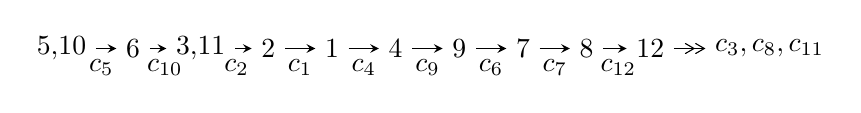
\begin{tikzpicture}[x=23pt, y=7pt]
	% node
	\node (A0) at (-1/8, 0) {5,10};
	\node (A1) at (1, 0) {6};
	\node (A2) at (33/16, 0) {3,11};
	\node (A3) at (25/8, 0) {2};
	\node (A4) at (33/8, 0) {1};
	\node (A5) at (41/8, 0) {4};
	\node (A6) at (49/8, 0) {9};
	\node (A7) at (57/8, 0) {7};
	\node (A8) at (65/8, 0) {8};
	\node (A9) at (73/8, 0) {12};
	\node (C1) at (1/2, -1) {$c_{5}$};
	\node (C2) at (3/2, -1) {$c_{10}$};
	\node (C3) at (21/8, -1) {$c_{2}$};
	\node (C4) at (29/8, -1) {$c_{1}$};
	\node (C5) at (37/8, -1) {$c_{4}$};
	\node (C6) at (45/8, -1) {$c_{9}$};
	\node (C7) at (53/8, -1) {$c_{6}$};
	\node (C8) at (61/8, -1) {$c_{7}$};
	\node (C9) at (69/8, -1) {$c_{12}$};
	\node (A10) at (11, 0) {$c_{3},c_{8},c_{11}$};

	% edge
	\draw[->,>=stealth]	
	(A0) edge (A1) (A1) edge (A2) (A2) edge (A3) (A3) edge (A4) (A4) edge (A5) (A5) edge (A6) (A6) edge (A7) (A7) edge (A8) (A8) edge (A9) ;
	\draw[->>,>={angle 60}]	
	(A9) edge (A10);
\end{tikzpicture} \\ 

\end{tabular} \\

\footnotetext{
The image of knot diagram is generated by the software ``\textbf{Draw programme}" developed by Andrew Bartholomew(\url{http://www.layer8.co.uk/maths/draw/index.htm\#Running-draw}), where we modified some parts for our purpose(\url{https://github.com/CATsTAILs/LinksPainter}).
}\phantom \\ \newline 
\centering \textbf{Ideals for irreducible components\footnotemark of $X_{\text{par}}$} 
 
\begin{align*}
I^u_{1}&=\langle 
3.05834\times10^{15} u^{34}-7.90175\times10^{15} u^{33}+\cdots+2.09912\times10^{16} b+1.74277\times10^{16},\\
\phantom{I^u_{1}}&\phantom{= \langle  }7.98092\times10^{16} u^{34}-1.40145\times10^{17} u^{33}+\cdots+6.29736\times10^{16} a+1.13113\times10^{17},\;u^{35}-2 u^{34}+\cdots+2 u-1\rangle \\
I^u_{2}&=\langle 
b+1,\;4 u^4-3 u^3+16 u^2+3 a-8 u+10,\;u^5- u^4+4 u^3-3 u^2+3 u-1\rangle \\
\\
\end{align*}
\raggedright * 2 irreducible components of $\dim_{\mathbb{C}}=0$, with total 40 representations.\\
\footnotetext{All coefficients of polynomials are rational numbers. But the coefficients are sometimes approximated in decimal forms when there is not enough margin.}
\newpage
\renewcommand{\arraystretch}{1}
\centering \section*{I. $I^u_{1}= \langle 3.06\times10^{15} u^{34}-7.90\times10^{15} u^{33}+\cdots+2.10\times10^{16} b+1.74\times10^{16},\;7.98\times10^{16} u^{34}-1.40\times10^{17} u^{33}+\cdots+6.30\times10^{16} a+1.13\times10^{17},\;u^{35}-2 u^{34}+\cdots+2 u-1 \rangle$}
\flushleft \textbf{(i) Arc colorings}\\
\begin{tabular}{m{7pt} m{180pt} m{7pt} m{180pt} }
\flushright $a_{5}=$&$\begin{pmatrix}1\\0\end{pmatrix}$ \\
\flushright $a_{10}=$&$\begin{pmatrix}0\\u\end{pmatrix}$ \\
\flushright $a_{6}=$&$\begin{pmatrix}1\\u^2\end{pmatrix}$ \\
\flushright $a_{3}=$&$\begin{pmatrix}-1.26734 u^{34}+2.22546 u^{33}+\cdots-0.810928 u-1.79619\\-0.145696 u^{34}+0.376432 u^{33}+\cdots-1.05037 u-0.830238\end{pmatrix}$ \\
\flushright $a_{11}=$&$\begin{pmatrix}- u\\u\end{pmatrix}$ \\
\flushright $a_{2}=$&$\begin{pmatrix}-1.41304 u^{34}+2.60189 u^{33}+\cdots-1.86130 u-2.62643\\-0.145696 u^{34}+0.376432 u^{33}+\cdots-1.05037 u-0.830238\end{pmatrix}$ \\
\flushright $a_{1}=$&$\begin{pmatrix}-0.375032 u^{34}+0.960289 u^{33}+\cdots-0.228111 u-1.08728\\0.0296343 u^{34}-0.108392 u^{33}+\cdots-0.0371536 u-0.0245560\end{pmatrix}$ \\
\flushright $a_{4}=$&$\begin{pmatrix}-1.24493 u^{34}+2.18658 u^{33}+\cdots-1.42273 u-1.62947\\-0.161215 u^{34}+0.434551 u^{33}+\cdots-1.04853 u-0.806713\end{pmatrix}$ \\
\flushright $a_{9}=$&$\begin{pmatrix}u\\u^3+u\end{pmatrix}$ \\
\flushright $a_{7}=$&$\begin{pmatrix}u^2+1\\u^4+2 u^2\end{pmatrix}$ \\
\flushright $a_{8}=$&$\begin{pmatrix}-0.367678 u^{34}+0.886943 u^{33}+\cdots-0.895712 u-0.926179\\0.0213029 u^{34}-0.0716902 u^{33}+\cdots-1.30130 u+0.337244\end{pmatrix}$ \\
\flushright $a_{12}=$&$\begin{pmatrix}-0.367678 u^{34}+0.886943 u^{33}+\cdots-0.895712 u-0.926179\\0.0222806 u^{34}-0.0350461 u^{33}+\cdots+0.630447 u-0.185658\end{pmatrix}$\\&\end{tabular}
\flushleft \textbf{(ii) Obstruction class $= -1$}\\~\\
\flushleft \textbf{(iii) Cusp Shapes $= \frac{111368899656244763}{188920669770572085} u^{34}-\frac{254954201870553542}{188920669770572085} u^{33}+\cdots+\frac{234691530598543088}{37784133954114417} u-\frac{1174662391668223564}{188920669770572085}$}\\~\\
\newpage\renewcommand{\arraystretch}{1}
\flushleft \textbf{(iv) u-Polynomials at the component}\newline \\
\begin{tabular}{m{50pt}|m{274pt}}
Crossings & \hspace{64pt}u-Polynomials at each crossing \\
\hline $$\begin{aligned}c_{1}\end{aligned}$$&$\begin{aligned}
&u^{35}+40 u^{34}+\cdots+11466 u+81
\end{aligned}$\\
\hline $$\begin{aligned}c_{2},c_{4}\end{aligned}$$&$\begin{aligned}
&u^{35}-6 u^{34}+\cdots+102 u-9
\end{aligned}$\\
\hline $$\begin{aligned}c_{3},c_{7}\end{aligned}$$&$\begin{aligned}
&u^{35}-3 u^{34}+\cdots+768 u+288
\end{aligned}$\\
\hline $$\begin{aligned}c_{5},c_{6},c_{9}\\c_{10}\end{aligned}$$&$\begin{aligned}
&u^{35}-2 u^{34}+\cdots+2 u-1
\end{aligned}$\\
\hline $$\begin{aligned}c_{8},c_{11}\end{aligned}$$&$\begin{aligned}
&u^{35}+2 u^{34}+\cdots-2 u-1
\end{aligned}$\\
\hline $$\begin{aligned}c_{12}\end{aligned}$$&$\begin{aligned}
&u^{35}+24 u^{34}+\cdots+12 u+1
\end{aligned}$\\
\hline
\end{tabular}\\~\\
\newpage\renewcommand{\arraystretch}{1}
\flushleft \textbf{(v) Riley Polynomials at the component}\newline \\
\begin{tabular}{m{50pt}|m{274pt}}
Crossings & \hspace{64pt}Riley Polynomials at each crossing \\
\hline $$\begin{aligned}c_{1}\end{aligned}$$&$\begin{aligned}
&y^{35}-84 y^{34}+\cdots+90434070 y-6561
\end{aligned}$\\
\hline $$\begin{aligned}c_{2},c_{4}\end{aligned}$$&$\begin{aligned}
&y^{35}-40 y^{34}+\cdots+11466 y-81
\end{aligned}$\\
\hline $$\begin{aligned}c_{3},c_{7}\end{aligned}$$&$\begin{aligned}
&y^{35}+33 y^{34}+\cdots+935424 y-82944
\end{aligned}$\\
\hline $$\begin{aligned}c_{5},c_{6},c_{9}\\c_{10}\end{aligned}$$&$\begin{aligned}
&y^{35}+36 y^{34}+\cdots+12 y-1
\end{aligned}$\\
\hline $$\begin{aligned}c_{8},c_{11}\end{aligned}$$&$\begin{aligned}
&y^{35}-24 y^{34}+\cdots+12 y-1
\end{aligned}$\\
\hline $$\begin{aligned}c_{12}\end{aligned}$$&$\begin{aligned}
&y^{35}-24 y^{34}+\cdots+308 y-1
\end{aligned}$\\
\hline
\end{tabular}\\~\\
\newpage\flushleft \textbf{(vi) Complex Volumes and Cusp Shapes}
$$\begin{array}{c|c|c}  
\text{Solutions to }I^u_{1}& \I (\text{vol} + \sqrt{-1}CS) & \text{Cusp shape}\\
 \hline 
\begin{aligned}
u &= \phantom{-}0.823932 + 0.577808 I \\
a &= -0.155370 - 0.797556 I \\
b &= \phantom{-}1.65857 - 0.14735 I\end{aligned}
 & -11.98490 + 3.28428 I & -11.99097 - 0.69750 I \\ \hline\begin{aligned}
u &= \phantom{-}0.823932 - 0.577808 I \\
a &= -0.155370 + 0.797556 I \\
b &= \phantom{-}1.65857 + 0.14735 I\end{aligned}
 & -11.98490 - 3.28428 I & -11.99097 + 0.69750 I \\ \hline\begin{aligned}
u &= -0.845135 + 0.556282 I \\
a &= \phantom{-}0.064458 + 0.876271 I \\
b &= \phantom{-}1.57251 - 0.09566 I\end{aligned}
 & -7.58978 + 2.78007 I & -9.93716 - 2.70438 I \\ \hline\begin{aligned}
u &= -0.845135 - 0.556282 I \\
a &= \phantom{-}0.064458 - 0.876271 I \\
b &= \phantom{-}1.57251 + 0.09566 I\end{aligned}
 & -7.58978 - 2.78007 I & -9.93716 + 2.70438 I \\ \hline\begin{aligned}
u &= \phantom{-}0.826909 + 0.535223 I \\
a &= \phantom{-}0.160633 - 1.094940 I \\
b &= \phantom{-}1.67277 + 0.32231 I\end{aligned}
 & -12.1055 - 8.7330 I & -11.74675 + 5.60158 I \\ \hline\begin{aligned}
u &= \phantom{-}0.826909 - 0.535223 I \\
a &= \phantom{-}0.160633 + 1.094940 I \\
b &= \phantom{-}1.67277 - 0.32231 I\end{aligned}
 & -12.1055 + 8.7330 I & -11.74675 - 5.60158 I \\ \hline\begin{aligned}
u &= -0.219192 + 0.760543 I \\
a &= \phantom{-}0.413862 + 0.000591 I \\
b &= \phantom{-}0.381823 + 0.140239 I\end{aligned}
 & \phantom{-}1.26028 + 2.02659 I & -0.48961 - 4.26135 I \\ \hline\begin{aligned}
u &= -0.219192 - 0.760543 I \\
a &= \phantom{-}0.413862 - 0.000591 I \\
b &= \phantom{-}0.381823 - 0.140239 I\end{aligned}
 & \phantom{-}1.26028 - 2.02659 I & -0.48961 + 4.26135 I \\ \hline\begin{aligned}
u &= -0.107525 + 1.257610 I \\
a &= \phantom{-}1.49280 - 1.31844 I \\
b &= -1.77830 + 0.61280 I\end{aligned}
 & -2.63751 + 2.36122 I & -11.77236 - 2.92931 I \\ \hline\begin{aligned}
u &= -0.107525 - 1.257610 I \\
a &= \phantom{-}1.49280 + 1.31844 I \\
b &= -1.77830 - 0.61280 I\end{aligned}
 & -2.63751 - 2.36122 I & -11.77236 + 2.92931 I\\
 \hline 
 \end{array}$$\newpage$$\begin{array}{c|c|c}  
\text{Solutions to }I^u_{1}& \I (\text{vol} + \sqrt{-1}CS) & \text{Cusp shape}\\
 \hline 
\begin{aligned}
u &= \phantom{-}0.048161 + 1.339420 I \\
a &= \phantom{-}0.150468 + 1.217930 I \\
b &= -1.223220 - 0.264994 I\end{aligned}
 & \phantom{-}2.04451 - 1.19616 I & -3.22654 + 0.68114 I \\ \hline\begin{aligned}
u &= \phantom{-}0.048161 - 1.339420 I \\
a &= \phantom{-}0.150468 - 1.217930 I \\
b &= -1.223220 + 0.264994 I\end{aligned}
 & \phantom{-}2.04451 + 1.19616 I & -3.22654 - 0.68114 I \\ \hline\begin{aligned}
u &= \phantom{-}0.537614 + 0.278615 I \\
a &= -0.194970 + 0.880512 I \\
b &= -0.777018 - 1.038680 I\end{aligned}
 & -4.08309 - 3.66975 I & -13.2607 + 6.9860 I \\ \hline\begin{aligned}
u &= \phantom{-}0.537614 - 0.278615 I \\
a &= -0.194970 - 0.880512 I \\
b &= -0.777018 + 1.038680 I\end{aligned}
 & -4.08309 + 3.66975 I & -13.2607 - 6.9860 I \\ \hline\begin{aligned}
u &= \phantom{-}0.07172 + 1.41763 I \\
a &= \phantom{-}1.40227 + 1.58971 I \\
b &= -0.568896 - 0.136236 I\end{aligned}
 & \phantom{-}2.34289 - 0.25916 I & -8.00000 - 1.73801 I \\ \hline\begin{aligned}
u &= \phantom{-}0.07172 - 1.41763 I \\
a &= \phantom{-}1.40227 - 1.58971 I \\
b &= -0.568896 + 0.136236 I\end{aligned}
 & \phantom{-}2.34289 + 0.25916 I & -8.00000 + 1.73801 I \\ \hline\begin{aligned}
u &= \phantom{-}0.18444 + 1.40762 I \\
a &= \phantom{-}0.09162 + 2.08933 I \\
b &= -0.46414 - 1.41482 I\end{aligned}
 & \phantom{-}1.31340 - 6.28579 I & -8.00000 + 6.17936 I \\ \hline\begin{aligned}
u &= \phantom{-}0.18444 - 1.40762 I \\
a &= \phantom{-}0.09162 - 2.08933 I \\
b &= -0.46414 + 1.41482 I\end{aligned}
 & \phantom{-}1.31340 + 6.28579 I & -8.00000 - 6.17936 I \\ \hline\begin{aligned}
u &= -0.13397 + 1.43446 I \\
a &= \phantom{-}0.24966 - 1.49398 I \\
b &= -0.263513 + 0.834456 I\end{aligned}
 & \phantom{-}5.13989 + 3.03126 I & \phantom{-0.000000 } 0. - 3.33629 I \\ \hline\begin{aligned}
u &= -0.13397 - 1.43446 I \\
a &= \phantom{-}0.24966 + 1.49398 I \\
b &= -0.263513 - 0.834456 I\end{aligned}
 & \phantom{-}5.13989 - 3.03126 I & \phantom{-0.000000 -}0. + 3.33629 I\\
 \hline 
 \end{array}$$\newpage$$\begin{array}{c|c|c}  
\text{Solutions to }I^u_{1}& \I (\text{vol} + \sqrt{-1}CS) & \text{Cusp shape}\\
 \hline 
\begin{aligned}
u &= -0.544097\phantom{ +0.000000I} \\
a &= -0.567908\phantom{ +0.000000I} \\
b &= -1.72921\phantom{ +0.000000I}\end{aligned}
 & -6.34482\phantom{ +0.000000I} & -17.4700\phantom{ +0.000000I} \\ \hline\begin{aligned}
u &= -0.383769 + 0.315386 I \\
a &= \phantom{-}0.415262 - 1.043400 I \\
b &= -0.449868 + 0.371769 I\end{aligned}
 & -0.534568 + 1.131870 I & -6.35643 - 6.10930 I \\ \hline\begin{aligned}
u &= -0.383769 - 0.315386 I \\
a &= \phantom{-}0.415262 + 1.043400 I \\
b &= -0.449868 - 0.371769 I\end{aligned}
 & -0.534568 - 1.131870 I & -6.35643 + 6.10930 I \\ \hline\begin{aligned}
u &= \phantom{-}0.273233 + 0.399953 I \\
a &= \phantom{-}3.06116 + 1.12201 I \\
b &= -0.847017 + 0.385254 I\end{aligned}
 & -3.28792 + 0.94378 I & -10.44072 + 4.60691 I \\ \hline\begin{aligned}
u &= \phantom{-}0.273233 - 0.399953 I \\
a &= \phantom{-}3.06116 - 1.12201 I \\
b &= -0.847017 - 0.385254 I\end{aligned}
 & -3.28792 - 0.94378 I & -10.44072 - 4.60691 I \\ \hline\begin{aligned}
u &= \phantom{-}0.30180 + 1.54032 I \\
a &= -0.90061 - 1.57197 I \\
b &= \phantom{-}1.62707 + 0.48300 I\end{aligned}
 & -5.36857 - 12.88450 I & \phantom{-0.000000 } 0 \\ \hline\begin{aligned}
u &= \phantom{-}0.30180 - 1.54032 I \\
a &= -0.90061 + 1.57197 I \\
b &= \phantom{-}1.62707 - 0.48300 I\end{aligned}
 & -5.36857 + 12.88450 I & \phantom{-0.000000 } 0 \\ \hline\begin{aligned}
u &= -0.31717 + 1.54997 I \\
a &= -0.84603 + 1.20335 I \\
b &= \phantom{-}1.51007 - 0.28880 I\end{aligned}
 & -0.76082 + 7.07720 I & \phantom{-0.000000 } 0 \\ \hline\begin{aligned}
u &= -0.31717 - 1.54997 I \\
a &= -0.84603 - 1.20335 I \\
b &= \phantom{-}1.51007 + 0.28880 I\end{aligned}
 & -0.76082 - 7.07720 I & \phantom{-0.000000 } 0 \\ \hline\begin{aligned}
u &= \phantom{-}0.30705 + 1.57204 I \\
a &= -1.108790 - 0.870354 I \\
b &= \phantom{-}1.56930 + 0.03692 I\end{aligned}
 & -4.96905 - 0.92386 I & \phantom{-0.000000 } 0\\
 \hline 
 \end{array}$$\newpage$$\begin{array}{c|c|c}  
\text{Solutions to }I^u_{1}& \I (\text{vol} + \sqrt{-1}CS) & \text{Cusp shape}\\
 \hline 
\begin{aligned}
u &= \phantom{-}0.30705 - 1.57204 I \\
a &= -1.108790 + 0.870354 I \\
b &= \phantom{-}1.56930 - 0.03692 I\end{aligned}
 & -4.96905 + 0.92386 I & \phantom{-0.000000 } 0 \\ \hline\begin{aligned}
u &= -0.393303\phantom{ +0.000000I} \\
a &= \phantom{-}1.22750\phantom{ +0.000000I} \\
b &= \phantom{-}0.0923140\phantom{ +0.000000I}\end{aligned}
 & -0.995121\phantom{ +0.000000I} & -10.5770\phantom{ +0.000000I} \\ \hline\begin{aligned}
u &= -0.06492 + 1.66171 I \\
a &= -0.365988 - 0.087264 I \\
b &= \phantom{-}0.749270 + 0.127452 I\end{aligned}
 & \phantom{-}9.76537 + 3.12159 I & \phantom{-0.000000 } 0 \\ \hline\begin{aligned}
u &= -0.06492 - 1.66171 I \\
a &= -0.365988 + 0.087264 I \\
b &= \phantom{-}0.749270 - 0.127452 I\end{aligned}
 & \phantom{-}9.76537 - 3.12159 I & \phantom{-0.000000 } 0 \\ \hline\begin{aligned}
u &= \phantom{-}0.331033\phantom{ +0.000000I} \\
a &= -3.18710\phantom{ +0.000000I} \\
b &= -1.10194\phantom{ +0.000000I}\end{aligned}
 & -2.12637\phantom{ +0.000000I} & -0.370270\phantom{ +0.000000I}\\
 \hline 
 \end{array}$$\newpage\newpage\renewcommand{\arraystretch}{1}
\centering \section*{II. $I^u_{2}= \langle b+1,\;4 u^4-3 u^3+16 u^2+3 a-8 u+10,\;u^5- u^4+4 u^3-3 u^2+3 u-1 \rangle$}
\flushleft \textbf{(i) Arc colorings}\\
\begin{tabular}{m{7pt} m{180pt} m{7pt} m{180pt} }
\flushright $a_{5}=$&$\begin{pmatrix}1\\0\end{pmatrix}$ \\
\flushright $a_{10}=$&$\begin{pmatrix}0\\u\end{pmatrix}$ \\
\flushright $a_{6}=$&$\begin{pmatrix}1\\u^2\end{pmatrix}$ \\
\flushright $a_{3}=$&$\begin{pmatrix}-\frac{4}{3} u^4+u^3+\cdots+\frac{8}{3} u-\frac{10}{3}\\-1\end{pmatrix}$ \\
\flushright $a_{11}=$&$\begin{pmatrix}- u\\u\end{pmatrix}$ \\
\flushright $a_{2}=$&$\begin{pmatrix}-\frac{4}{3} u^4+u^3+\cdots+\frac{8}{3} u-\frac{13}{3}\\-1\end{pmatrix}$ \\
\flushright $a_{1}=$&$\begin{pmatrix}-1\\0\end{pmatrix}$ \\
\flushright $a_{4}=$&$\begin{pmatrix}-\frac{4}{3} u^4+u^3+\cdots+\frac{8}{3} u-\frac{10}{3}\\-1\end{pmatrix}$ \\
\flushright $a_{9}=$&$\begin{pmatrix}u\\u^3+u\end{pmatrix}$ \\
\flushright $a_{7}=$&$\begin{pmatrix}u^2+1\\u^4+2 u^2\end{pmatrix}$ \\
\flushright $a_{8}=$&$\begin{pmatrix}u^2+1\\u^4+2 u^2\end{pmatrix}$ \\
\flushright $a_{12}=$&$\begin{pmatrix}- u^2-1\\u^2\end{pmatrix}$\\&\end{tabular}
\flushleft \textbf{(ii) Obstruction class $= 1$}\\~\\
\flushleft \textbf{(iii) Cusp Shapes $= -\frac{58}{9} u^4+\frac{13}{3} u^3-\frac{211}{9} u^2+\frac{128}{9} u-\frac{223}{9}$}\\~\\
\newpage\renewcommand{\arraystretch}{1}
\flushleft \textbf{(iv) u-Polynomials at the component}\newline \\
\begin{tabular}{m{50pt}|m{274pt}}
Crossings & \hspace{64pt}u-Polynomials at each crossing \\
\hline $$\begin{aligned}c_{1},c_{2}\end{aligned}$$&$\begin{aligned}
&(u-1)^5
\end{aligned}$\\
\hline $$\begin{aligned}c_{3},c_{7}\end{aligned}$$&$\begin{aligned}
&u^5
\end{aligned}$\\
\hline $$\begin{aligned}c_{4}\end{aligned}$$&$\begin{aligned}
&(u+1)^5
\end{aligned}$\\
\hline $$\begin{aligned}c_{5},c_{6}\end{aligned}$$&$\begin{aligned}
&u^5- u^4+4 u^3-3 u^2+3 u-1
\end{aligned}$\\
\hline $$\begin{aligned}c_{8}\end{aligned}$$&$\begin{aligned}
&u^5- u^4+u^2+u-1
\end{aligned}$\\
\hline $$\begin{aligned}c_{9},c_{10},c_{12}\end{aligned}$$&$\begin{aligned}
&u^5+u^4+4 u^3+3 u^2+3 u+1
\end{aligned}$\\
\hline $$\begin{aligned}c_{11}\end{aligned}$$&$\begin{aligned}
&u^5+u^4- u^2+u+1
\end{aligned}$\\
\hline
\end{tabular}\\~\\
\newpage\renewcommand{\arraystretch}{1}
\flushleft \textbf{(v) Riley Polynomials at the component}\newline \\
\begin{tabular}{m{50pt}|m{274pt}}
Crossings & \hspace{64pt}Riley Polynomials at each crossing \\
\hline $$\begin{aligned}c_{1},c_{2},c_{4}\end{aligned}$$&$\begin{aligned}
&(y-1)^5
\end{aligned}$\\
\hline $$\begin{aligned}c_{3},c_{7}\end{aligned}$$&$\begin{aligned}
&y^5
\end{aligned}$\\
\hline $$\begin{aligned}c_{5},c_{6},c_{9}\\c_{10},c_{12}\end{aligned}$$&$\begin{aligned}
&y^5+7 y^4+16 y^3+13 y^2+3 y-1
\end{aligned}$\\
\hline $$\begin{aligned}c_{8},c_{11}\end{aligned}$$&$\begin{aligned}
&y^5- y^4+4 y^3-3 y^2+3 y-1
\end{aligned}$\\
\hline
\end{tabular}\\~\\
\newpage\flushleft \textbf{(vi) Complex Volumes and Cusp Shapes}
$$\begin{array}{c|c|c}  
\text{Solutions to }I^u_{2}& \I (\text{vol} + \sqrt{-1}CS) & \text{Cusp shape}\\
 \hline 
\begin{aligned}
u &= \phantom{-}0.233677 + 0.885557 I \\
a &= \phantom{-}0.162657 + 0.410020 I \\
b &= -1.00000\phantom{ +0.000000I}\end{aligned}
 & \phantom{-}0.17487 - 2.21397 I & -9.00284 + 4.40290 I \\ \hline\begin{aligned}
u &= \phantom{-}0.233677 - 0.885557 I \\
a &= \phantom{-}0.162657 - 0.410020 I \\
b &= -1.00000\phantom{ +0.000000I}\end{aligned}
 & \phantom{-}0.17487 + 2.21397 I & -9.00284 - 4.40290 I \\ \hline\begin{aligned}
u &= \phantom{-}0.416284\phantom{ +0.000000I} \\
a &= -3.11537\phantom{ +0.000000I} \\
b &= -1.00000\phantom{ +0.000000I}\end{aligned}
 & -2.52712\phantom{ +0.000000I} & -22.8010\phantom{ +0.000000I} \\ \hline\begin{aligned}
u &= \phantom{-}0.05818 + 1.69128 I \\
a &= \phantom{-}0.728361 + 0.139255 I \\
b &= -1.00000\phantom{ +0.000000I}\end{aligned}
 & \phantom{-}9.31336 - 3.33174 I & -11.48557 + 5.79761 I \\ \hline\begin{aligned}
u &= \phantom{-}0.05818 - 1.69128 I \\
a &= \phantom{-}0.728361 - 0.139255 I \\
b &= -1.00000\phantom{ +0.000000I}\end{aligned}
 & \phantom{-}9.31336 + 3.33174 I & -11.48557 - 5.79761 I\\
 \hline 
 \end{array}$$\newpage
\newpage\renewcommand{\arraystretch}{1}
\centering \section*{ III. u-Polynomials}
\begin{tabular}{m{50pt}|m{274pt}}
Crossings & \hspace{64pt}u-Polynomials at each crossing \\
\hline $$\begin{aligned}c_{1}\end{aligned}$$&$\begin{aligned}
&((u-1)^5)(u^{35}+40 u^{34}+\cdots+11466 u+81)
\end{aligned}$\\
\hline $$\begin{aligned}c_{2}\end{aligned}$$&$\begin{aligned}
&((u-1)^5)(u^{35}-6 u^{34}+\cdots+102 u-9)
\end{aligned}$\\
\hline $$\begin{aligned}c_{3},c_{7}\end{aligned}$$&$\begin{aligned}
&u^5(u^{35}-3 u^{34}+\cdots+768 u+288)
\end{aligned}$\\
\hline $$\begin{aligned}c_{4}\end{aligned}$$&$\begin{aligned}
&((u+1)^5)(u^{35}-6 u^{34}+\cdots+102 u-9)
\end{aligned}$\\
\hline $$\begin{aligned}c_{5},c_{6}\end{aligned}$$&$\begin{aligned}
&(u^5- u^4+4 u^3-3 u^2+3 u-1)(u^{35}-2 u^{34}+\cdots+2 u-1)
\end{aligned}$\\
\hline $$\begin{aligned}c_{8}\end{aligned}$$&$\begin{aligned}
&(u^5- u^4+u^2+u-1)(u^{35}+2 u^{34}+\cdots-2 u-1)
\end{aligned}$\\
\hline $$\begin{aligned}c_{9},c_{10}\end{aligned}$$&$\begin{aligned}
&(u^5+u^4+4 u^3+3 u^2+3 u+1)(u^{35}-2 u^{34}+\cdots+2 u-1)
\end{aligned}$\\
\hline $$\begin{aligned}c_{11}\end{aligned}$$&$\begin{aligned}
&(u^5+u^4- u^2+u+1)(u^{35}+2 u^{34}+\cdots-2 u-1)
\end{aligned}$\\
\hline $$\begin{aligned}c_{12}\end{aligned}$$&$\begin{aligned}
&(u^5+u^4+4 u^3+3 u^2+3 u+1)(u^{35}+24 u^{34}+\cdots+12 u+1)
\end{aligned}$\\
\hline
\end{tabular}\newpage\renewcommand{\arraystretch}{1}
\centering \section*{ IV. Riley Polynomials}
\begin{tabular}{m{50pt}|m{274pt}}
Crossings & \hspace{64pt}Riley Polynomials at each crossing \\
\hline $$\begin{aligned}c_{1}\end{aligned}$$&$\begin{aligned}
&((y-1)^5)(y^{35}-84 y^{34}+\cdots+90434070 y-6561)
\end{aligned}$\\
\hline $$\begin{aligned}c_{2},c_{4}\end{aligned}$$&$\begin{aligned}
&((y-1)^5)(y^{35}-40 y^{34}+\cdots+11466 y-81)
\end{aligned}$\\
\hline $$\begin{aligned}c_{3},c_{7}\end{aligned}$$&$\begin{aligned}
&y^5(y^{35}+33 y^{34}+\cdots+935424 y-82944)
\end{aligned}$\\
\hline $$\begin{aligned}c_{5},c_{6},c_{9}\\c_{10}\end{aligned}$$&$\begin{aligned}
&(y^5+7 y^4+16 y^3+13 y^2+3 y-1)(y^{35}+36 y^{34}+\cdots+12 y-1)
\end{aligned}$\\
\hline $$\begin{aligned}c_{8},c_{11}\end{aligned}$$&$\begin{aligned}
&(y^5- y^4+4 y^3-3 y^2+3 y-1)(y^{35}-24 y^{34}+\cdots+12 y-1)
\end{aligned}$\\
\hline $$\begin{aligned}c_{12}\end{aligned}$$&$\begin{aligned}
&(y^5+7 y^4+16 y^3+13 y^2+3 y-1)(y^{35}-24 y^{34}+\cdots+308 y-1)
\end{aligned}$\\
\hline
\end{tabular}
\vskip 2pc
\end{document}